\chapter{Обзор современного состояния бортовых оптико-электронных систем специального назначения} \label{ch:ch1}

Обзор современного состояния бортовых оптико-электронных систем специального назначения разделен на несколько частей:
\begin{enumerate}
  \item Обзорно-поисковые, прицельные и пилотажные оптико-электронные системы;
  \item Авиационные оптико-электронные системы инфракрасного противодействия ракетной атаке;
  \item Анализ способов обеспечения обратной связи в современных ОЭС.
\end{enumerate}

В современных условиях применения в предполагаемых локальных и региональных военных конфликтах обычного вооружения важнейшую роль играют ЛА тактической военной авиации самолеты, вертолеты и БЛА. Они являются одним из основных средств борьбы с предполагаемым наземным, надводным и воздушным противником. При этом существенным требованием является ведение ими предполагаемых боевых действий круглосуточно, в простых и сложных метеоусловиях. 

Одним из основных компонентов бортового радиоэлектронного оборудования вышеуказанных ЛА являются ОЭ обзорно-поисковые 
(рисунок \ref{fig:soep}) и прицельные системы, обеспечивающие более высокую точность по сравнению с радиолокационными системами, особенно при работе по наиболее "трудным" для них малоразмерным наземным целям на пестрых земных фонах. В свою очередь, пилотажные оптико-электронные системы обеспечивают маловысотное пилотирования военных ЛА к району ведения боевых действий с обходом находящихся по курсу полета препятствий с целью снижения своей видимости радиолокационными средствами ПВО противника.

\begin{figure}[ht]
  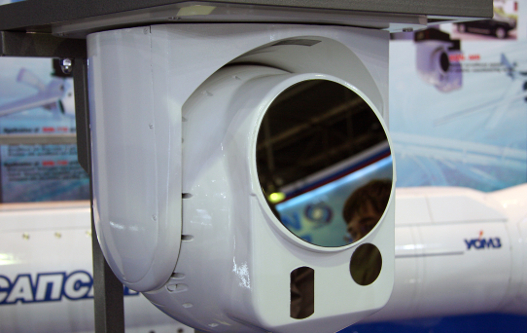
\includegraphics[width=1.0\linewidth]{p1} 
  \caption{Оптико-электронная система СОН-730}
  \label{fig:soep}
\end{figure}

Радикальным преимуществом оптико-электронных систем по сравнению с радиолокационными является также и гораздо более высокая скрытность их работы, что существенно повышает выживаемость ЛА в ходе проведения ими боевых действий. 

Однако у этих систем есть большой недостаток по сравнению с радиолокационными существенная зависимость их рабочих характеристик от метеоусловий и невозможность работы через облачность. 

По реализуемым ТТХ многие отечественные авиационные ОЭС, к сожалению, отстают от современного мирового уровня. Это обусловлено, главным образом, более низким качеством отечественной оптико-электронной элементной базы для них и технологического производственного оборудования. Важным фактором достижения успешного конкурентоспособного результата является следование строгой методике разработки и исследования динамики вновь разрабатываемых систем управления бортовыми оптико-электронными приборами, использование информационных технологий для ускорения разработки изделий и уменьшения количества ошибок. Отсутствие процесса моделирования системы управления во время разработки прибора может снижать общую надежность изделия.

Крайне важно видеть наиболее перспективные направления совершенствования отечественной оптико-электронной техники выбирая наиболее перспективные направления как по степени их приоритетности, так и по минимуму технических рисков. 

В этой связи для разработчиков и потребителей отечественных ЛА значительный интерес представляют данные по серийным авиационным оптико-электронным системам, используемым в настоящее время в зарубежной авиационной практике. Одновременно для них представляют интерес и тенденции совершенствования этих систем с тем, чтобы знать, на что можно рассчитывать в ближайшем будущем и в каких именно направлениях нам самим целесообразно продвигаться дальше. 

Целью данного обзора является представление информации по этим вопросам, а также сравнительный анализ представленных систем по критерию выполняемой боевой задачи. 

\section{Обзорно-поисковые, прицельные и пилотажные оптико-электронные системы} \label{sec:ch1/sec1-}

Для создания ОЭС смотрящего типа базирующейся на ЛА рассмотрим некоторые аналогичные приборы зарубежного и Российского производства. Таблица \ref{tab:EOS} демонстрирует зарубежные и российские авиационные обзорно-поисковые, прицельных и пилотажных оптико-электронных систем (ОЭС), произведенные за последние 10 лет. 

\begin{landscape}

\begin{longtable}{| p{6cm} | p{18cm} |}
	\caption{Поисково-следящие системы авиационного базирования}%
	\label{tab:EOS}% label всегда желательно идти после caption
	\\ \hline
		Название комплекса, 
		
		Страна производитель, 
		
		Год начала производства, 
		
		Масса 
		& 
		Описание 
	\\ \hline
		OSF (Optronique Secteur Frontal). Thales Optronics, SAGEM, \cite[]{OSF}
		
		Франция, 
		
		2010 г., 
		
		95 кг.    
	& 
		ДТВ, 3-5 + 8-12 мкм-IRST, ЛД-1,54. Установлена в верхней носовой части самолета перед кабиной з фюзеляжа выведены 2 раздельные IRST- и ДТВ + ЛД-головки. Последняя является ОМБ ОП-подсистемы "CIU" (Combat Identification Unit), предназначенной как для наведения на воздушные цели УР "воздух-воздух", так и для решения прицельных задач по земле, воде. 
		IRST-подсистема обеспечивает круглосуточное обнаружение и распознавание воздушных целей, имеет ТпВ-режим. Фотоматериал и топология используемых в ней фоточувствительных элементов не сообщаются (по косвенным данным, в обоих диапазонах используются сканирующие 4х288 эл.-субматрицы). 
		
		
		Днем для более точного распознавания и идентификации этих целей используется узкопольный ДТВ из состава ОП-подсистемы "CIU". Со временем планируется заменить его на круглосуточную ТВ-камеру. По имеющимся данным, дальность обнаружения воздушных целей IRST-подсистемой составляет Rо 80...100 км, ДТВ 30...50 км, типовых наземных целей соответственно 40 (в ТпВ-режиме) и 35 км. 
		
		Основную же нагрузку при решении ударных задач по земле, воде несет уже приводившаяся ранее, также предназначенная для использования на самолете Rafale контейнерная ОПС "DAMOCLES".
	\\ \hline
		IR OTIS. Saab Bofors Dynamics \cite[]{doi:10.1117/12.450557},
		
		Швеция	
		
		2010 г,	
		
		30-10 кг
		           
	& 
		Встроенная 8-12 мкм-IRST + ОП-система для шведского самолета Jas 39 Gripen. 
		Данная система предназначена для работы по воздуху и земле. В ней используется сканирующий фотоприемник с числом элементов nэл 1200, фоточувствительный материал и топология расположения элементов не сообщаются (по косвенным данным, это 4х288 эл-КРТ-субматрица). Она может работать 30 как с широкими полями зрения для быстрого обзора, так и с узкими для обнаружения целей на больших дальностях. Опять же по косвенным данным, эти поля равны 12х12 / 5,5х5,5 / 2х2о. 
		Сектора обзора могут выставляться оператором в заданных направлениях в пределах передней полусферы самолета. Система может работать в IPST-режиме сразу по многим целям "на проходе" и в ТпВ-режиме осуществлять точное АС выбранной цели. 
		ОМБ установлен на верхней носовой части фюзеляжа самолета, перед кабиной, несколько левее строительной оси самолета для обеспечения ограниченного обзора земной поверхности. 
		  
	\\ \hline
		Strix / Nightowl. SAGEM	
		
		Франция	
		
		2000 г. 	
		
		105 кг        
	&  
		Для французского экскортного вертолета Tigre HAP. Надкабинное размещение, также может наводить на цели ПТУР "HOT" и "Hellfire". 
		Оптический визир (ОВ), 3х-польные ДТВ, 8-12 мкм-ТпВ-II, ЛД-1,54, ИК-пеленгатор ПТУР "HOT", 
		может быть ЛДЦ-1,06 / 1,54, ПЛП. Может наводиться на цели от НСЦИ пилота. В ТпВ используется сканирующая 4х288 эл.-КРТ-субматрица, миниЭЛТ вводит ДТВ- и ТпВ-изображения в окуляр ОВ (возможна модификация и без ОВ). 
		При изготовлении корпуса ОМБ этой ОПС используются облегченные композитные материалы, что 
		крайне важно для надкабинного конструктивного исполнения.
		   
	\\ \hline
		M-TADS / PNVS. Lockheed Martin, DRS Technologies
		\cite[]{lockheedmartin}
		
		США	
		
		2005 г. 
		        
	& 
		ОП + пилотажная ОЭС американского армейского вертолета AH-64D Apache Longbow. Носовое размещение. 
		В состав ОП-подсистемы "M-TADS" входят ч/б ДТВ, 3-5 мкм-ТпВ-III, 8-12 мкм-ТпВ-II, ЛДЦ-1,06 / 1,54, ПЛП, ИНС / GPS, в состав пилотажной подсистемы "M-PNVS" широкопольные НУТВ и 8-12 мкм-ТпВ-II. 
		В 8-12 мкм-ТпВ-II-каналах обеих подсистем используются сканирующие 4х480 эл.-КРТ-субматрицы, 
		в 3-5 мкм-ТпВ-III-канале ОП-подсистемы смотрящая 320х256 эл.-InSb-матрица + микроскан (nэл
		экв= 640х512). Последний размещен в одном отсеке с ДТВ, при этом отсек имеет прозрачное для обоих этих каналов сапфировое входное окно. 
		В обеих подсистемах предусмотрены интегрирование ТВ- и ТпВ-изображений, выдача их на НСЦИ 
		пилотов и, в оцифрованном виде, на землю и на другие ЛА.
		    
	\\ \hline
		CоMPASS.		
		
		2001 г. 	
		
		38 - 35 кг      
& 
Панкратический ч/б или цветной ДТВ, 3х-польный 3-5 мкм-ТпВ-III, ЛД-1,54 или ЛЦУ-1,06, ПЛП, 0,8 
мкм-лазерный маркер. Может быть 8-12 мкм-ТпВ-II. В 3-5 мкм-ТпВ используется 320х256 эл.-InSb-матрица + микроскан (nэлэкв = 640х512), он может быть 
панкратическим. В 8-12 мкм-ТпВ используются сканирующая 4х288 эл.-КРТ-субматрица и дискретные 
поля зрения. ЛД-1,54 на Er-стекле, в ЛЦУ-1,06 используется ППЛ-накачка. Его энергия в импульсе Еи 80 мДж, частота повторения Fи 20 Гц. Мощность излучения маркера Ризл 50 мВт. 
    
\\ \hline
		D-CоMPASS.
				
		2005 г. 
			
		32 - 41 кг      
& 
Могут быть ч/б или цветной ДТВ, 3-5 мкм-ТпВ-III, 8-12 мкм-ТпВ-II, ЛД-1,54, ЛДЦ-1,06 / 1,54 с ППЛ- 
накачкой его лазерного излучателя, ПЛП, 0,8 мкм-лазерный маркер, ИНС / GPS-блок. 
Варианты ДТВ: 
панкратические ч/б или цветной,  панкратический цветной, на более крупноформатной (1,3 мп) матрице,  широкопольный с полем зрения по горизонтали г = 24о. 
Варианты ТпВ: 
3-5 мкм-ТпВ-III на 640х512 эл.-InSb-матрице, с фиксированными полями зрения ( у = 0,67х 0,5о),  то же самое, но с панкратическим изменением промежуточных i ,  3-5 мкм-ТпВ-III на 320х256 эл.-InSb-матрице, с более широкими i ,  8-12 мкм-ТпВ-II на сканирующей 4х288 эл.-КРТ-субматрице, с более широкими i . 
ИНС / GPS-блок обеспечивает высокоточную навигацию ЛА, задаваемые режимы обзора пространства, выработку абсолютных координат (геолокацию) целей, многоканальное их АС 
. Видеоизображения и символика могут выдаваться на ИЛС или на НСЦИ пилота. 
    
\\ \hline
	SEOS. Saab Bofors Dynamics \cite[]{doi:10.1117/12.450557}
	
	Швеция	
	
	2005 г. 	
	
	70 кг	      
& 
ДТВ, 8-12 мкм-ТпВ-II, ЛД-1,54. Могут быть НУТВ, 3-5 мкм-ТпВ-III, ИК-пеленгатор ПТУР, ЛЦУ-
1,06, лазерно-лучевой канал управления (ЛЛКУ) ПТУР.
Есть улучшение качества и интегрирование между собой ДТВ- и ТпВ-изображений.
   
\\ \hline
		OLOSP. SAGEM
		\cite[]{sagem-olosp}
		
		Франция		25 кг
		 
		40 кг. 
		       
& 
Могут быть панкратический цветной ДТВ, высокоразрешающий ч/б ДТВ, 3-5 мкм-ТпВ-III, 8-12 мкм-ТпВ-II, ЛД-1,54, радиолиния передачи информации на землю. 
ДТВ построен по 3х-матричной схеме формирования цветности, 3-5 мкм-ТпВ на 640х512 эл.-КРТ-матрице, 8-12 мкм-ТпВ на сканирующей 4х288 эл.-КРТ-субматрице. 
   
\\ \hline
		EUROFLIR 410. SAGEM
		\cite[]{EUROFLIR}
		Франция, Technobit, Испания	2008 г	45 кг
		       
& 
Модульная система. Могут быть различные варианты с панкратическими мегапиксельным цветным 
ДТВ, ч/б НУТВ, 3-5 мкм-ТпВ-III или 8-12 мкм-ТпВ-II, 0,15о
-спотоскопом, ЛД-1,54, ЛЦУ-1,06, 0,8 мкм-лазерным маркером. 3-5 мкм-ТпВ на 640х512 эл.-КРТ-матрице, 8-12 мкм-ТпВ на сканирующей 4х288 эл.-КРТ-субматрице.
   
\\ \hline
		FIN 1010 AN / AAR-51. Selex Galileo	
		
		Англия		     
& 
Для самолетов английских ВВС и американского Корпуса морской пехоты (КМП). Может использоваться также и на военно-транспортных и гражданских самолетах. Может быть в контейнерном и во встроенном конструктивных исполнениях. 
В ТпВ используется 8 эл.-КРТ SPRITE, = 25х16о, ТпВ-изображение выводится на кабинный ИЛС. 
   
\\ \hline
		Pathfinder. Lockheed Martin	
		
		США		
		
		90 кг.       
& 
Создан на базе навигационного контейнера "AN / AAQ-13" довольно популярной в прошлом самолет-
ной ОП + пилотажной ОЭС "LANTIRN" с исключением из него 3 см-навигационой РЛС. 
Так же, как и раньше, в ТпВ используется сканирующая однорядная 180 эл.-КРТ-линейка, в отличие 
от ТпВ упомянутого контейнера теперь используется не одно, а 2 поля зрения ш / у = 28х21 / 9х7о
, уз-
кое поле предназначено для обнаружения наземных целей.     
\\ \hline
		Sure Sight EVS. CMC Electronics Inc.	
		
		США	2001 г	
		
		8,2-1,8 кг
		        
& 
Эта система (Enhanced Vision System) предназначена для использования на борту военно-транспортных и гражданских бизнес-самолетов с целью обеспечения круглосуточного "видения" их пилотами обстановки в аэропорту при взлете-посадке, маневрировании на земле в условиях ухудшенной видимости (ночью, в осадках, тумане и т.п.). 
Сначала в этой системе использовался только ТпВ-канал, потом, в качестве опции, был добавлен мм-рл-канал. ТпВ размещен в обтекателе метеоРЛС, "смотрит" вперед через ИК-прозрачное окно. Может быть размещен и под или над обтекателем мм-рл-канала. ТпВ- и рл-изображения в проинтегрированном (синтезированном) виде выводятся на самолетный ИЛС. Есть 2 варианта построения ТпВ-канала: - 8-12 мкм-ТпВ-II на криогенно охлаждаемой сканирующей 4х288 эл-КРТ-субматрице, имеет высокую чувствительность, дает качественное изображение, масса m = 8,2 кг, 
-более дешевый 8-14 мкм-ТпВ-III на неохлаждаемой 320х240 эл.-матрице, m = 1,8 кг, может размещаться в носу ЛА или быть встроен его хвостовое оперение.
    
\\ \hline
		PACIS. Selex Galileo
		
		Англия		
		
		33 кг        
& 
Помимо пилотажных задач может решать и прицельные. Используется 8 эл.-КРТ-SPRITE, поля зрения ш / у = 40х30 / 10х6,6о, кадровая частота Fк = 25 Гц/   
\\ \hline
	AN / AAQ-18. Raytheоn	
	
	США		       
& 
Используется сканирующая 120 эл.-КРТ-линейка, ш / у = 18х14 / 4х3о   
\\ \hline
	Pathfinder. Lockheed Martin	
	
	США	
	
	2009 г.	
	
	50 кг        
& 
Для транспортных вертолетов общего назначения CH-47 Chinook и UH-60 Black Hawk. Устанавливается в носу вертолета.
Данная ОЭС была создана на базе пилотажной подсистемы "M-PNVS" американского боевого вертолета AH-64D Apache Longbow по разд.2. В ТпВ-канале используется сканирующая 4х480 эл.-КРТ-субматрица, разворачиваемая в две горизонтальные полосы с формированием в кадре N = 1728х960 элементов разложения (пикселей). Поле зрения равно = 52х30о. НУТВ- и ТпВ-изображения интегрируются между собой и выдаются на НСЦИ пилота. НУТВ может "видеть" искусственные световые источники, что облегчает пилотаж, а также подсвет от сухопутных лазерных маркеров, что улучшает взаимодействие с СВ. 
    
\\ \hline
	NOCTUA. Thales Optronics	
	
	Англия, Cumulus, ЮАР		
	
	24,5 кг       
& 
Для южноафриканского боевого вертолета Rooivalk. Используется сканирующая 4х288 эл-КРТ-субматрица, = 40х30о, ТпВ-изображение выдается на НСЦИ пилота, управляющую визирной осью ТпВ со ср. кв. ошибкой 18'.     
\\ \hline
	FLIR III. AIM	
	
	Германия		
	
	20 кг.       
& 
Для немецких вертолетов Tiger, NH 90 TTH. Используется сканирующая 4х288 эл-КРТ-субматрица, = 40х30о, ТпВ-изображение выдается на НСЦИ пилота.     
\\ \hline

\end{longtable}

\end{landscape}

По приведенным в таблице данным можно сделать некоторые выводы: 

\begin{enumerate}
	\item Опыт проведения странами НАТО боевых действий в ряде военных кампаний последних лет показал целесообразность возложения на обзорно-поисковые и прицельные ОЭС- самолетов, вертолетов и БЛА не только собственно разведывательно-прицельных задач, но и информационной поддержки своих наземных подразделений СВ и ВМС в части обеспечения их большей осведомленности относительно поведения противника в зоне проводимых ими боевых действий.
	\item С этой целью в состав оборудования ОЭС в последние годы стали включать лазерные маркеры для выдачи ЦУ наземным пользователям при ведении боевых действий в темное время суток. Сами же ЛА стали оснащаться линиями передачи изображений высокой четкости, на другие ЛА, участвующие вместе с ними в совместных боевых операциях, и т.п.
	\item В настоящее время наметилась устойчивая тенденция оснащения авиационных ОЭС датчиками высокого разрешения, имеющими ряд существенных технических и тактических достоинств. Так, они позволяют: использовать в этих датчиках менее габаритную (более короткофокусную) оптику; обеспечивать более высокие вероятностные характеристики обнаружения объектов; сократить временные затраты на распознавание последних. 
	\item Наиболее популярными в авиационных ОЭС ТпВ-датчиками являются:
	\begin{enumerate}
		\item 3...5-мкм ТпВ 3-го поколения (ТпВ-III) на не сканирующих ("смотрящих") матрицах на криогенно охлаждаемых антимониде индия (InSb) и кадмии-ртуть-теллуре (КРТ); 
		\item 8...12 мкм ТпВ 2-го поколения (ТпВ-II) на сканирующих КРТ-субматрицах, реже 8...12-мкм ТпВ-III на смотрящих КРТ-матрицах и еще реже 8...9-мкм ТпВ-III на смотрящих матрицах на арсениде галлия (GaAs); 
		 
		
		\item 8...12-мкм ТпВ-III на неохлаждаемых матрицах (чаще всего используются при решении наблюдательных задач).
	\end{enumerate}
	\item На боевых вертолетах сухопутной поддержки, зачастую работающих в условиях помех и разрывов боеприпасов на поле боя, преобладающими являются 8...12-мкм ТпВ-датчики, особенно если вертолеты предназначены для эксплуатации как в теплых, так и в холодных климатических зонах. В наиболее совершенных ОЭС используются оба спектральных диапазона. 
	\item На всех типах ЛА все большую популярность в последние годы приобретают панкратические цветные ДТВ, такие же ТпВ, сверхузкопольные ДТВ (спотоскопы), а лазерные маркеры. 
	\item Использование спотоскопов и маркеров стало возможным благодаря реализации в уникальных точностей стабилизации линий визирования входящих в их состав прицельных каналов (стаб 1...20") .
	\item В плане проведения модернизаций авиационных ОЭС следует предусматривать осуществление следующих технических мероприятий: 
	\begin{enumerate}
		\item переход в самолетных интегрированных ОЭС от контейнерного на встроенное конструктивное исполнение; 
		\item перевод лазерных излучателей ЛД, ЛЦУ с широкополосной ламповой на гораздо более эффективную по промышленному кпд узкополосную полупроводниковую накачку; 
		\item интегрирование между собой ДТВ-, НУТВ- и ТпВ-изображений; 
		\item применение вторичной цифровой обработки выходных видеосигналов этих датчиков с целью улучшения качества выдаваемых ими изображений перед предъявлением их летчикам, а также формирование по ним некоторого нового изображения с использованием преимуществ каждого из датчиков в той или иной обстановке; 
		\item введение в состав ОЭС собственных, инерциально-навигационных системных блоков для повышения точностей углового автосопровождения целей
		\item при использовании информации от бортовых GPS-приемников и ЛД, выдачи высокоточных координат этих целей в систему управления оружием "дальней руки", другим внешним по отношению к ЛА потребителям.  
	\end{enumerate}
\end{enumerate}

\section{Авиационные оптико-электронные системы инфракрасного противодействия ракетной атаке} \label{sec:ch1/sec2-}

Для излучающей ОЭС базирующейся на ЛА также рассмотрим некоторые аналогичные приборы зарубежного и Российского производства. Далее приведены зарубежные и российские авиационные оптико-электронные системы инфракрасного противодействия ракетной атаке. Можно выделить 3 поколения систем постановки оптико-электронных помех (СОЭП):

\begin{enumerate}
	\item Системы всенаправленной постановки помех
	\item Системы с узконаправленным пучком постановки помех
	\item Лазерные системы противодействия 	
\end{enumerate}

В состав системы противодействия ракетной атаке входят несколько подсистем. Состав расписан на рисунке \ref{fig:classification}.

\begin{figure}[ht]
	\centering
	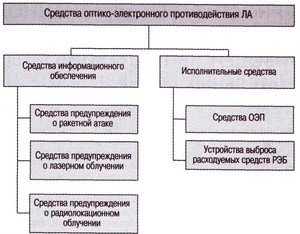
\includegraphics[width=0.6\linewidth]{p2} 
	\caption{Классификация средств СОЭП ЛА}
	\label{fig:classification}
\end{figure}

В составе исполнительных средств указаны “средства ОЭП”, система управления для этой подсистемы комплекса рассматривается в настоящей работе. Генератор пульсирующих инфракрасных помех представляет собой мощную инфракрасную лампу с вращающимся отражателем или способную изменять свою яркость с заданной частотой, в кожухе из прозрачного для инфракрасного излучения материала.

Ракеты с инфракрасной головкой самонаведения относятся к самым простым управляемым средствам поражения воздушных целей. Принцип сканирования поля зрения ГСН показан на рисунке \ref{fig:rocketScanning}. 

\begin{figure}[ht]
	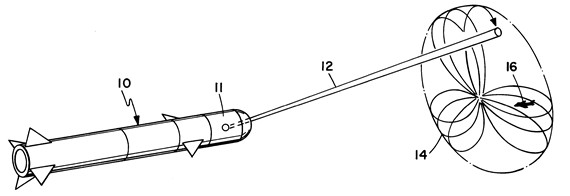
\includegraphics[width=1.0\linewidth]{p3} 
	\caption{Принцип сканирования головкой самонаведения ракеты}
	\label{fig:rocketScanning}
\end{figure}

\begin{itemize}
	\item 10 – ракета с ГСН
	\item 11 – сканирующая система в составе ГСН
	\item 12 – сектор моментального поля зрения
	\item 14 – полное поле зрения ГСН
	\item 16 – цель (летательный аппарат)	
\end{itemize}
	
При генерировании пульсирующих инфракрасных помех с частотой, равной рабочей частоте внутренних элементов наведения, и мощностью, сопоставимой с естественным тепловым излучением защищаемой цели, в систему наведения ракеты вносится помеха, приводящая к отклонению ракеты от защищаемой цели. Вероятность срыва атаки ракеты ПЗРК при использовании генераторов пульсирующих инфракрасных помех составляет от 0,5 до 0,7-0,8.

\subsection{СОЭП первого поколения}	

К СОЭП первого поколения относятся системы ненаправленной постановки помех. Такие системы не представляют интереса для проводимой работы так как не имеют системы наведения. Принцип действия станции основан на генерации всенаправленного модулированного помехового ИК-излучения со специальной структурой сигнала. К таким системам относятся \cite[]{SOEP_LIPA}:

\begin{itemize}
	\item «Липа» (РФ)	
	\item AN/ALQ-144 (США, смотри рисунок \ref{fig:alq})	
	\item AN/ALQ-157 by BAE Systems, used for larger helicopters and aircraft.
	\item AN/ALQ-212 by BAE Systems, currently fielded on U.S. Army CH-47 Chinook helicopters.
	\item “Адрос КТ-01 АВ” (Украина)
	\item “Квадрос-КМ-01 В” (Украина) 		
\end{itemize}

\begin{figure}[ht]
	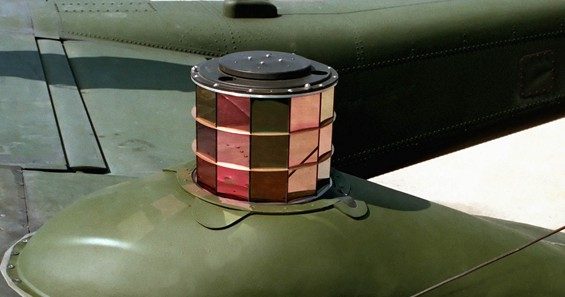
\includegraphics[width=1.0\linewidth]{p4} 
	\caption{СОЭП первого поколения}
	\label{fig:alq}
\end{figure}
\todo{редактировать рисунок, пояснения что где}

СОЭП первого поколения обеспечивают защиту военной авиационной техники от ракетных комплексов с инфракрасными головками самонаведения (ИК ГСН) типа «Сайдуиндер», «Ред Ай», «Чапарэл», «Питон», «Стрела-2М», «Хунинь-5» и им подобных. 

\subsection{СОЭП второго поколения}	

К СОЭП второго поколения относятся системы с узконаправленным модулированным пучком помехового излучения. Примеры приведены на рисунках ниже (рисунок \ref{fig:p6}, рисунок \ref{fig:p7}).

Принцип работы СОЭП узконаправленным пучком основан на раннем обнаружении пуска ракеты, ее сопровождении и подавлении канала наведения с использованием узконаправленного потока модулированного ИК излучения.  Работа средств направленного оптико-электронною противодействия ракетной атаке осуществляется в следующей последовательности (смотри рисунок \ref{fig:p5})[]:

\begin{enumerate}
	\item Обнаружение атакующей УР средствами информационного обеспечения в диапазонах 0,01-0,4 мкм (УФ) и 4-14 мкм (ИК).
	\item ОЭП ИК ГСН, формирование ложного сигнала от цели. 
	\item Срыв наведения на цель. 
	\item Цель вне поля зрения ГСН УР. 
	\item УР не представляет угрозы для вертолета.	
\end{enumerate}

\begin{figure}[ht]
	\centering
	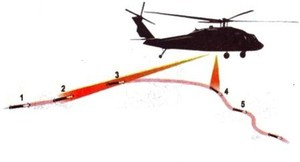
\includegraphics[width=0.7\linewidth]{p5} 
	\caption{Схема работы СОЭП при атаке ракетой с головкой самонаведения}
	\label{fig:p5}
\end{figure}

Использование нескольких излучателей, размещенных на ЛА, ЦСУ и оперативного перепрограммирования режимов работы значительно увеличивает вероятность противодействия угрозе ракетной атаки.

\begin{figure}[ht]
	\centering
	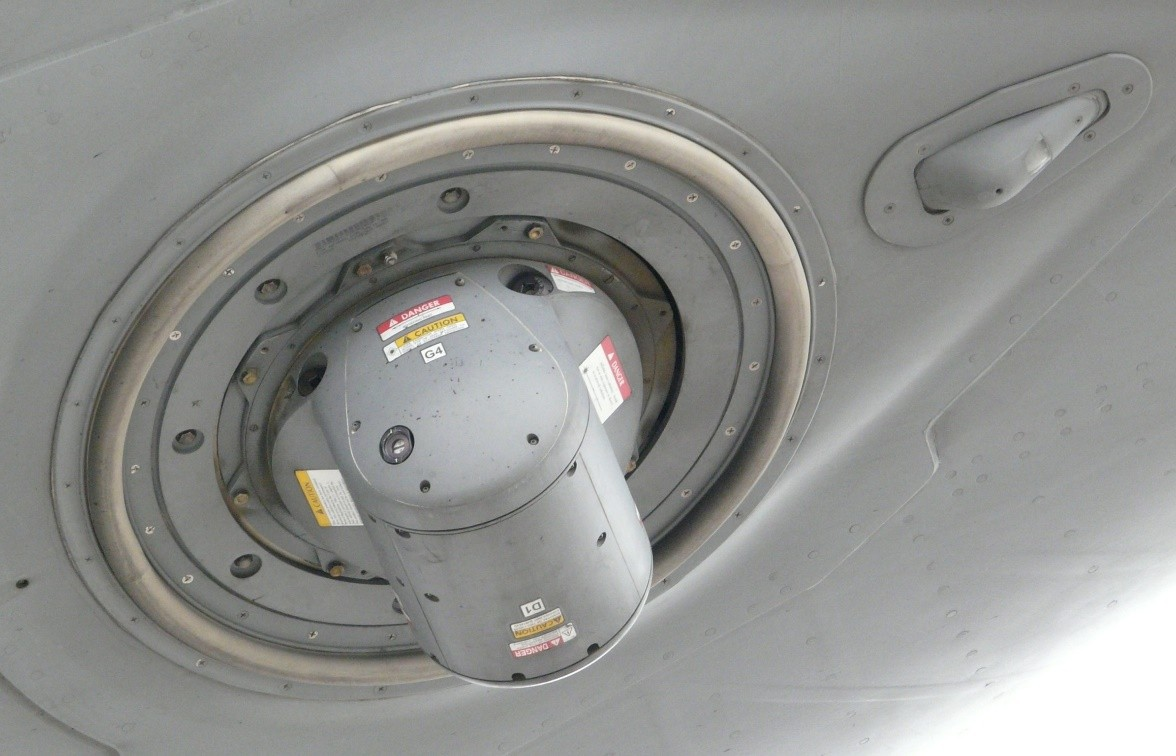
\includegraphics[width=0.8\linewidth]{p6} 
	\caption{СОЭП пульсирующих инфракрасных помех}
	\label{fig:p6}
\end{figure}

К СОЭП такого типа относятся \cite[]{Infrared_countermeasure}:
\begin{itemize}
	\item Президент-С;
	\item Leonardo’s Miysis DIRCM (directed infrared countermeasure);
	\item AN/AAQ-24 by Northrop Grumman – DIRCM;
	\item AN/ALQ-132 by Sanders/BAE Systems. Used in the 1960s in Vietnam, and was a fuel fired flashlamp system;
	\item CAMPS by Saab Avitronics, used for civilian and VIP aircraft;
	\item CIRCM by Northrop Grumman;
	\item Flight Guard by Israel Aerospace Industries, used in military and civilian aircraft (gain the nickname of "Live Saver" due to history of success in saving air vehicles during battles at several countries), but banned at several European airports. According to defense sources in Israel, the European ban is "odd and based mostly on a misunderstanding;
	\item ITT's CIRCM System;
	\item Selex ES' Miysis System;
	\item "Sukhogruz" - Russian DIRCM (used on Su-25T);
	\item KT-01 AVE and KT-02 ACE by Adron, used for military aircraft.		
\end{itemize}

\begin{figure}[ht]
	\centering
	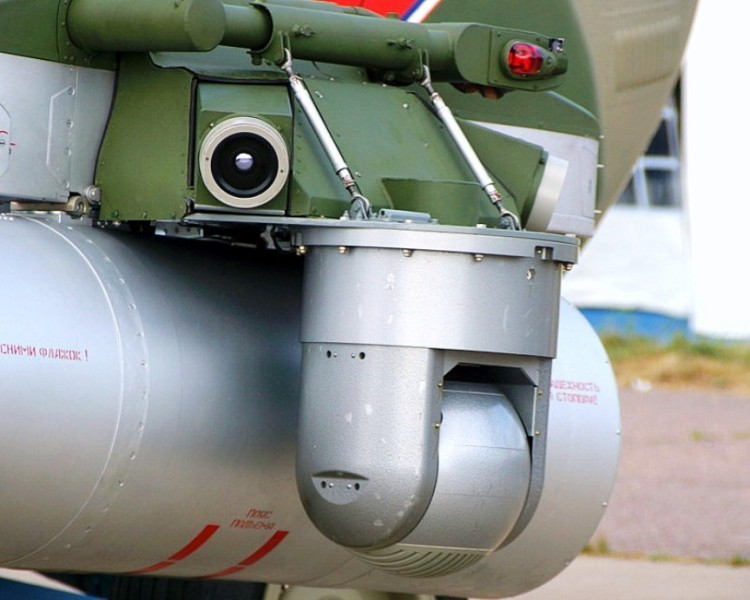
\includegraphics[width=0.6\linewidth]{p7} 
	\caption{Станция Л370-5 и УФ пеленгатор пуска ракет Л370-2}
	\label{fig:p7}
\end{figure}

\subsection{СОЭП третьего поколения}	
К СОЭП последнего поколения относятся лазерные системы защиты. Основными преимуществами таких систем являются независимость эффективности системы оптико-электронных помех от принципа работы головок наведения у ракет, меньший вес и габариты по сравнению с комплексами второго поколения. Визуальный облик показан на рисунке ниже (рисунок \ref{fig:p8}).

Одним из основных понятий физики взаимодействия лазерного излучения с веществом является порог разрушения. Принято различать два вида порогов – физический и технический. 

Физическим порогом разрушения материала называют такую плотность энергии или мощности (интенсивность) излучения, при которой происходят необратимые изменения оптических характеристик образца (пропускания, рассеяния, отражения) исследуемого материала. Изменение указанных характеристик является следствием образования разрушения, формирование которого сопровождается яркой вспышкой оптического излучения. 

\begin{figure}[ht]
	\centering
	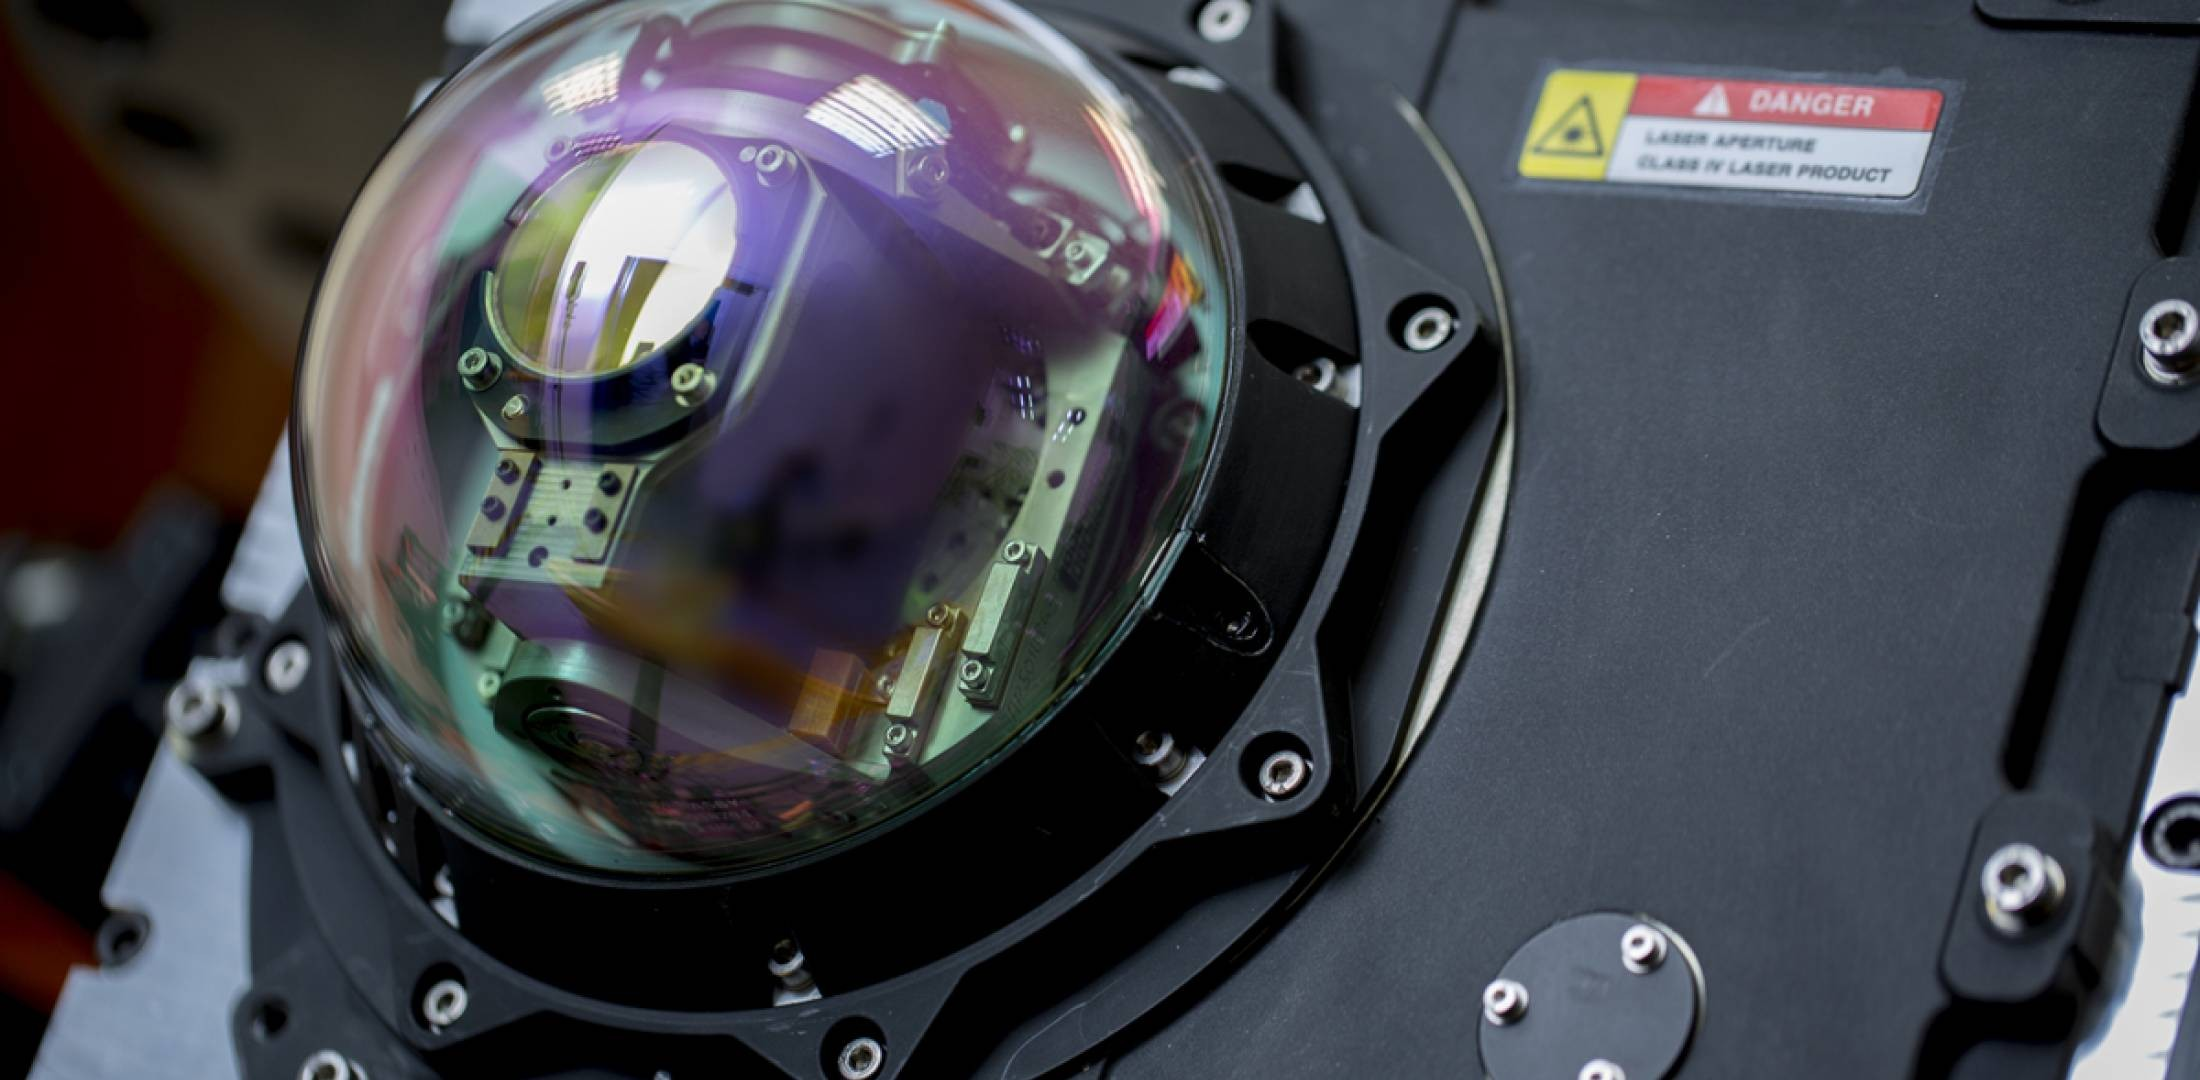
\includegraphics[width=0.8\linewidth]{p8} 
	\caption{Автоматическая бортовая лазерная станция постановки помех ALJS}
	\label{fig:p8}
\end{figure}

Техническим порогом разрушения называют такую плотность энергии или мощности излучения, при которой нарушается работоспособность изделия, изготовленного из исследуемого материала, вследствие изменений его оптических характеристик, превышающих допустимые.

Одним из немногих примеров комплексов третьего поколения является система MANTA (Испания). Это автоматическая бортовая лазерная станция постановки помех ALJS \cite[]{manta}.

Ее работа основывается на использовании кодированного мультиспектрального излучения импульсно-периодического (HF/DF) - лазера для создания помех в широком ИК-диапазоне.
Российский комплекс третьего поколения носит название Л370В28, его внешний вид показан на рисунке ниже (рисунок~\ref{fig:p9}). 

\begin{figure}[ht]
	\centering
	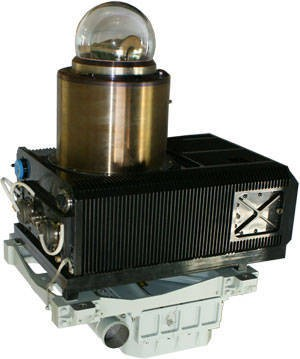
\includegraphics[width=0.5\linewidth]{p9} 
	\caption{Изделие Л370В28 (лазерная станция постановки помех)}
	\label{fig:p9}
\end{figure}

\section{Анализ способов обеспечения обратной связи в современных ОЭС} \label{sec:ch1/sec3-}

Для системы управления наиболее важным элементом является обратная связь. В автоматических оптико-электронных системах рассматриваемых типов управление происходит по углам наведения оптической оси, в качестве датчиков обратной связи углового положения используют следующие типы:
\begin{itemize}
	\item СКВТ (Синусно-косинусный вращающийся трансформатор)
	\todo{подробно}
	\item Датчик ХОЛЛА + датчик нуля (оптопара)
	\todo{подробно}
	\item Энкодер
	\todo{подробно}
\end{itemize}
С ростом технологичности электронной компонентной базы и появлением возможности обработки изображения в реальном времени для систем смотрящего типа обратную связь можно обеспечить обработкой информации с фотоприемника. Для этого используют:

\begin{itemize}
	\item \textbf{Одноэлементные фотоприемники с применением механических модуляторов}
	\todo{текст}
	\begin{figure}[ht]
		\centering
		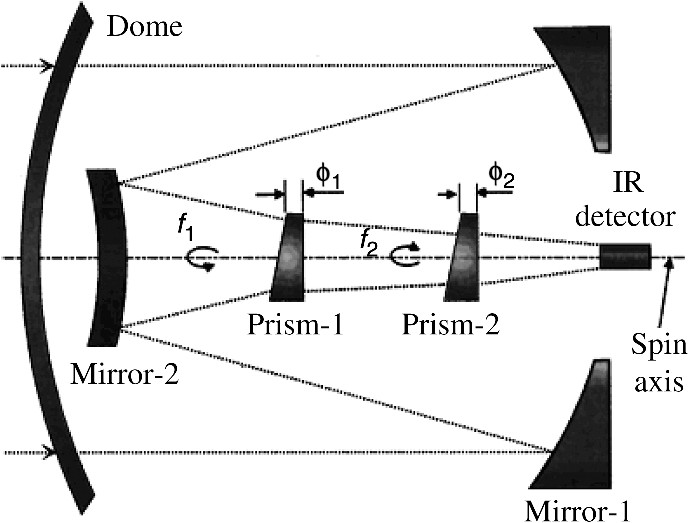
\includegraphics[width=0.6\linewidth]{p10} 
		\caption{Оптическая схема одноэлементной сканирующей ГСН  }
		\label{fig:p10}
	\end{figure}
	\item \textbf{позиционно чувстительные фотоприемники}
	Приемное устройство представляет собой четырехквадратный фотодиод. определение отклонения изображения объекта происходит путем вычисления разницы напряжений между элементами. 
	
	\todo{картинка}
	
	\item \textbf{Многоэлементные матричные фотоприемники}
	ПЗС-матрица — специализированная аналоговая интегральная микросхема, состоящая из светочувствительных фотодиодов, выполненная на основе кремния, использующая технологию ПЗС — приборов с зарядовой связью.
	
	ПЗС-матрицы выпускаются и активно используются компаниями Nikon, Canon, Sony, Fujitsu, Kodak, Matsushita, Philips и многими другими. В России ПЗС-матрицы сегодня разрабатывают и выпускают: ОАО «ЦНИИ „Электрон“» (г. Санкт-Петербург) и его дочернее предприятие ЗАО «НПП „Элар“» (г. Санкт-Петербург,) а также ОАО «НПП „Пульсар“» (г. Москва) \cite[]{CCD}.
	
	Наиболее приоритетный тип фотоприёмных устройств на данное время. Повсеместно используется в гражданской продукции, но для данной работы интересны ПЗС матрицы ИК спектра. Далее приведена сравнительная таблица с неохлаждаемыми доступными ПЗС матрицами ИК спектра на рынке.
	
	\todo{картинка}
\end{itemize}


\section{Выводы по главе} \label{sec:ch1/sec4-}

Бортовые оптико-электронные системы можно разделить на группы:
\begin{itemize}
	\item \textbf{Смотрящего типа}
	
	Характерными требованиями является точность позиционирования. На настоящий момент серийно производимые приборы достигают точности 10 угловых минут.
	
		
	\item \textbf{Излучающие}
	
	Характерным требованием является скорость наведения. На настоящий момент серийно производимые приборы обеспечивают скорости 700 градусов за секунду.
	\item \textbf{Мультиплексированные}
	
	
\end{itemize}

Ниже приведены основные характеристики бортовых оптико-электронных систем: 
\begin{itemize}
\item точность позиционирования  \todo{таблица}
\item скорость наведения
\item разрешение 
\item спектральный диапазон
\item частота опроса фотоприемника
\item рабочий сектор
\end{itemize}

Для каждого поколения СОЭП можно выделить свои особенности:
\begin{itemize}
	\item \textbf{Первого поколения}
	\begin{itemize}
		\item одновременное покрытие всей рабочей полусферы 
		\item простая конструкция
		\item малая мощность излучения
		\item малая глубина модуляции
		\item сильная привязка к типу подавляемой ракеты
	\end{itemize}
	\item \textbf{Второго поколения}
	\begin{itemize}
		\item большая мощность излучения
		\item возможность генерации различного типа модуляции
		\item более сложная конструкция
		\item малая точность наведения
		\item большая масса
	\end{itemize}
	\item \textbf{третьего поколения}
	\begin{itemize}
		\item работоспособность слабо зависит от типа подавляемой ракеты
		\item использование когерентного излучения
		\item малая ширина спектра излучения
		\item большая масса
		\item большая точнсть наведения
	\end{itemize}
\end{itemize}

Приведены основные способы обеспечения обратной связи в бортовых оптико-электронных системах:
\begin{itemize}
	\item \textbf{по управляющей координате}
	
	\begin{itemize}
		\item СКВТ (Синусно-косинусный вращающийся трансформатор)
		\item Датчик ХОЛЛА + датчик нуля (оптопара)
		\item Энкодер
	\end{itemize}
		
	\item \textbf{по сигналу с фотоприемника}
	
	\begin{itemize}
		\item Одноэлементные фотоприемники с применением механических модуляторов
		\item Позиционно чувстительные фотоприемники		
		\item Многоэлементные матричные фотоприемники	
	\end{itemize}
	
	
\end{itemize}

\todo{используются датчики положения привоов}

Важным этапом разработки любого изделия является создание математической модели, макетирование и моделирование динамики. Распространенной проблемой при разработке изделий является отсутствие методики разработки и исследования динамики систем управления бортовыми оптико-электронными приборами. Применение информационных технологий таких как CAD/CAM средства проектирования, средства математического моделирования (MATHCAD, MatLAB), средства контроля версий позволяют минимизировать человеческий фактор, а следование методике разработки позволяет обеспечить выполнение изначальных требований к проектируемому изделию. Решение вопросов такого характера обсуждается в главе \ref{ch:ch2}: \nameref{ch:ch2}.

\todo{Почему нужен оптимальный алгоритм управления БОЭП? }

отсутсвие оптимальной системы управления
в главе \ref{ch:ch4}: \nameref{ch:ch4}

 
\todo{Очень скромно. нужно привести их основные характеристики (преимущества и недостатки) связать их со своей работой, т.е. какие задачи остаются не решенные и какие необходимо решить в диссертации}
